\begin{center}
    \textbf{NEW NOTES FOR 02/26/25} \\
    \hrulefill
\end{center}

\section{The Neuron}

\begin{coloredlist}
    \item Definition: Basic information processing unit of the NS.
    \item Similarities to an animal cell:
    \begin{coloredlist}
        \item \cyanit{Cell membrane}: Separates the inside of the cell from the outside environment.
        \item \cyanit{Nucleus}: Contains the genetic material of the cell.
        \item \cyanit{Organelles}: Carry out the basic functions of the cell.
        \begin{coloredlist}
            \item \cyanit{Mitochondria}: Produce energy for the cell.
            \item \cyanit{Endoplasmic Reticulum}: Synthesizes proteins.
            \item \cyanit{Golgi Apparatus}: Packages proteins for transport.
            \item \cyanit{Lysosomes}: Break down waste products.
        \end{coloredlist}
        \item Basic cellular processes.
    \end{coloredlist}
    \item Differences:
    \begin{coloredlist}
        \item Special ``morphology'' (shape).
        \item Communicate through an electrochemical process.
    \end{coloredlist}
\end{coloredlist}

\subsection{Structure of the Neuron}
(Mostly a recap of \hyperref[Terms]{Terms})
\begin{coloredlist}
    \item \cyanit{Soma}
    \item \cyanit{Dendrite}
    \item \cyanit{Axon}
    \item \cyanit{Terminal Arboriza} -- Branches at the end of the axon.
    \item \cyanit{Terminal Buttons} -- End of the terminal arboriza.
    \item \cyanit{Axon Hillock}
    \item \cyanit{Myelin}
    \begin{coloredlist}
        \item Not all axons have it.
        \item Glial cells / 70\% Lipid / Nodes of Ranvier.
        \item Mutliple Sclerosis (MS) -- Demyelination.
    \end{coloredlist}
\end{coloredlist}

\subsection{Support cells in the Nervous System}

\begin{coloredlist}
    \item Glia/Glial Cells/ Neuroglia -- Support cells.
    \begin{coloredlist}
        \item Capable of cell division after birth/communication.
        \item Make up half of the volume, but are 10-50 times more numerous. (The other half is made up of neurons.)
        \item CNS:
        \begin{coloredlist}
            \item \cyanit{Macroglia} -- Large glial cells.
            \begin{coloredlist}
                \item \cyanit{Astrocytes} -- Star-shaped cells that provide physical support to neurons, clean up debris, and provide nutrients to neurons.
                \begin{coloredlist}
                    \item \textit{Note} that these cells do not help neurons grow when they are damaged. In fact, they inhibit growth by proliferating and forming a scar.
                \end{coloredlist}
                \item \cyanit{Oligodendrocytes} -- ``few branches (in contrast to Astrocytes)'' -- \textit{Form} myelin sheath around multiple axons in the CNS. 
            \end{coloredlist}
            \item \cyanit{Microglia} -- Small cells that remove debris from injured or dead cells.
            \item \cyanit{Ependymal Glia} -- Line the ventricles of the brain and spinal cord. (Remember the CSF?)
        \end{coloredlist}
        \item PNS:
        \begin{coloredlist}
            \item \cyanit{Satellite Cells} -- Provide nutrients and physical support to neurons.
            \item \cyanit{Schwann Cells} -- Form myelin sheath around axons in the PNS. These cells are monogamists; they wrap their arms around one axon.
            \begin{coloredlist}
                \item Neuronal Regeneration. 
            \end{coloredlist}
        \end{coloredlist}
        \item The Myelin Sheath is composed of Oligodendrocytes in the CNS and Schwann Cells in the PNS.
        \item \cyanit{Phagocytosis} -- When an injury occurs, the glial cells divide and eat the dead cells. (Done by Microglia and Schwann Cells.)
        \item Maintenance of Internal Consistency.
        \begin{coloredlist}
            \item When neurons undergo rapid firing, they release potassium ions. Astrocytes absorb these ions to maintain the internal consistency of the neuron, and dump them into the blood stream.
        \end{coloredlist}
    \end{coloredlist}
\end{coloredlist}

\begin{center}
    \textbf{NEW NOTES FOR 02/28/25} \\
    \hrulefill
\end{center}

\subsection{Are Glial Cells Contributing to Alzheimer's Disease?}

\begin{coloredlist}
    \item Normally,
    \begin{coloredlist}
        \item Beta amyloid cleared away through microglia.
    \end{coloredlist}
    \item IF beta amyloid builds up too much, Tau INSIDE cells builds up.
    \item This leads to inflammation, which maybe leads to the problems of Alzheimer's.
\end{coloredlist}

\section{Different Kinds of Neurons}

\begin{coloredlist}
    \item Based on Structure
    \item Based on Function
\end{coloredlist}

\subsection{Structural Classification of Neurons}

\begin{coloredlist}
    \item \cyanit{Unipolar/Pseudounipolar}
    \begin{coloredlist}
        \item \textit{The difference:} The axon and dendrite are fused together.
    \end{coloredlist}
    \item \cyanit{Bipolar}
    \item \cyanit{Multipolar}
\end{coloredlist}

\subsection{Functional Classification of Neurons}

\begin{coloredlist}
    \item Sensory Neurons (Afferent)
    \begin{coloredlist}
        \item Carry information from the sensory receptors to the CNS.
        \item Unipolar.
        \item ``Afferent'' -- ``bearing or conducting inward''
    \end{coloredlist}
    \item Interneurons
    \item Motor Neurons (Efferent)
    \begin{coloredlist}
        \item Carry information from the CNS to the muscles and glands.
        \item Multipolar.
        \item ``Efferent'' -- ``conducting outward''
    \end{coloredlist}
    \item Remember: \(\text{Ad = towards} \qquad \text{Ex = from} \qquad \text{Ferro = I carry}.\)
\end{coloredlist}

\section{Neural Communication}

\begin{coloredlist}
    \item \textbf{2 Systems of Neuronal Communication:}
    \begin{coloredlist}
        \item \cyanit{Binary} -- All or none (literally only 2 options).
        \item \cyanit{Analogue} --Graded, matter or degree.
    \end{coloredlist}
\end{coloredlist}

\begin{center}
    \textbf{NEW NOTES FOR 03/03/25 (kinda)} \\
    We added a lot to the notes that we already had, so there is new material springled throughout this section. \\
    \hrulefill
\end{center}

\subsection{Binary System (``Off'' and ``On'')}

\begin{coloredlist}
    \item \cyanit{The Resting Membrane Potential (RMP)}: ``OFF'' 
    \begin{coloredlist}
        \item \hyperref[resting potential]{Click here for a diagram.}
        \item \textit{Note:} Where the arrows land on either side of the cell membrane is supposed to represent the relative permeability of the cell membrane to different ions.
        \item -70 mV (relative to the outside).
        \item Understand the cell membrane.
        \begin{coloredlist}
            \item \cyanit{Phospholipid Bilayer} -- Hydrophobic tails and hydrophilic heads.
            \item \cyanit{Semipermeability} -- Some things can cross, others cannot.
            \begin{coloredlist}
                \item Lipid, lipid soluble, small, and neutral.
            \end{coloredlist}
            \item \cyanit{Embedded Proteins} -- Channels and pumps. 
            \begin{coloredlist}
                \item \textbf{4 Jobs We Care About:}
                \begin{coloredlist}
                    \item \cyanit{Receptors}
                    \begin{coloredlist}
                        \item High specificity and affinity.
                        \item ``Places where things can bind to the cell and cause a change.''
                    \end{coloredlist}
                    \item \cyanit{Channels}.
                    \begin{coloredlist}
                        \item \cyanit{Gated Channels}: 
                        \begin{coloredlist}
                            \item Passive movement. The cell itself does not expel any energy to move the ions.
                            \item Chemical (ligand) gated channels.
                            \item Voltage gated channels.
                        \end{coloredlist}
                    \end{coloredlist}
                    \item \cyanit{Pumps} -- Active transport.
                    \item \cyanit{Enzymes} -- Facilitates chemical reactions.
                    \begin{coloredlist}
                        \item Breaking neurochemicals down or putting them back together.
                    \end{coloredlist}
                \end{coloredlist}
            \end{coloredlist}
        \end{coloredlist}
        \item \textbf{3 Determinants of the RMP}
        \begin{coloredlist}
            \item \cyanit{Differential Permeability} -- The cell membrane is more permeable to some ions than others.
            \begin{coloredlist}
                \item For sodium, the membrane only allows a trickle of \(\text{Na}^{+}\) into the cell.
                \item Conversely, the membrane is more permeable to \(\text{K}^{+}\) and \(\text{CL}^{-}\). (\(\text{K}^{+}\) is the most permeable.)
            \end{coloredlist}
            \item \textbf{Driving Forces}:
            \begin{coloredlist}
                \item \cyanit{Diffusion} -- Ions move from high to low concentration (Concentration Gradient).
                \begin{coloredlist}
                    \item \textit{Note:} The cell membrane is more permeable to potassium ions than sodium ions.
                \end{coloredlist}
                \item \cyanit{Electrostatic Pressure} -- Ions move towards the opposite charge (Electrical Gradient).
                \item \cyanit{Equilibrium Potential} -- The charge the ion ``perfers'' if it were the only one and could pass freely through the membrane.
                \begin{coloredlist}
                    \item This answers the question: ``Why doesn't the cell get more and more negative?''
                    \item Driving force in (influx) = Driving force out (efflux).
                    \item \(\text{K}^+ = -80 \text{ mV}\) and \(\text{Na}^+ = +55 \text{ mV}\).
                \end{coloredlist}
            \end{coloredlist}
            \item \cyanit{Sodium-Potassium Pump} (\(\text{Na}^{+}\)/\(\text{K}^{+}\) Pump)
            \begin{coloredlist}
                \item 3 \(\text{Na}^{+}\) out for every 2 \(\text{K}^{+}\) in.
                \item Costs 1 ATP.
            \end{coloredlist}
        \end{coloredlist}
    \end{coloredlist}
    \item \cyanit{The Action Potential (AP)}: ``ON'' 
    \begin{coloredlist}
        \item \hyperref[action potential]{Click here for a diagram.}
        \begin{coloredlist}
            \item \textit{Note:} The above diagram neglects to show that there can be \textit{failed} attempts at an action potential wherein the threshold is not reached. In these cases, the charge of the cell can increase or decrease, but if it does not reach -55 mV, it will quickly settle back to its resting potential of -70 mV.
        \end{coloredlist}
        \item +40 mV (relative to the outside).
        \item Thus, during an action potential, there is a total of 110 mV difference between the inside and outside the cell.

        \begin{center}
            \textbf{NEW NOTES FOR 03/05/25} \\
            \hrulefill
        \end{center}
        \item \textbf{Electrical Current}
        \begin{coloredlist}
            \item \cyanit{Depolarization}
            \begin{coloredlist}
                \item A little 
                \item A lot
                \begin{coloredlist}
                    \item \cyanit{Threshold of Excitation} = +15 mV.
                    \item Action potential
                \end{coloredlist}
                \item Even more.
            \end{coloredlist}
            \item \cyanit{Repolarization}
            \begin{coloredlist}
                \item A little
                \item A lot
                \item Even more.
            \end{coloredlist}
        \end{coloredlist}
        \item \cyanit{Refractory Period}
        \begin{coloredlist}
            \item Cell is resistant to reexciation for a period after the AP peak.
            \begin{coloredlist}
                \item \cyanit{Absolute Refractory Period} -- No amount of stimulation will cause another AP.
                \item \cyanit{Relative Refractory Period} -- A stronger than normal stimulus is required to cause another AP. (This is because of hyperpolarization.)
            \end{coloredlist}
        \end{coloredlist}
        \item \textbf{Three Questions:}
        \begin{coloredlist}
            \item Why don't the \(\text{Na}^{+}\) channels reopen during repolarization? \checkmark
            \begin{coloredlist}
                \item \textit{Answer:} Because of the refractory period.
            \end{coloredlist}
            \item How can an all or none signal convey analog information? \checkmark
            \begin{coloredlist}
                \item \textit{Answer:} The frequency of the APs can convey the intensity of the stimulus.
                \item \cyanit{Rate Law} -- Variations in the intensity of a stimulus are represented by variations in the rate of firing.
            \end{coloredlist}
            \item Where does that signal come from that meets the threshold of excitation?
            \begin{coloredlist}
                \item \cyanit{Decremental Conduction} -- The further the signal travels, the weaker it gets. (cable properties)
                \begin{coloredlist}
                    \item Analogue communication.
                    \begin{coloredlist}
                        \item Degrading because for resistance and leakage.
                    \end{coloredlist}
                    \item \cyanit{Passive Conduction} -- No energy is expended.
                \end{coloredlist}
            \end{coloredlist}
        \end{coloredlist}
    \end{coloredlist}
\end{coloredlist}

\subsection{Conduction of Action Potential in Unmyelinated Axons}

\begin{center}
    \textbf{NEW NOTES FOR 03/07/25} \\
    \hrulefill
\end{center}

\begin{coloredlist}
    \item \cyanit{All or Nothing Law} -- AP occurs or not once triggered, always the same size.
    \item \cyanit{Active Regeneration} -- The AP is regenerated at each point along the axon.
    \begin{coloredlist}
        \item Takes a lot of time (\(<\) 1--10 meters/second).
        \item Takes a lot of energy.
    \end{coloredlist}
\end{coloredlist}

\subsection{Conduction of Action Potential in Myelinated Axons}

\begin{coloredlist}
    \item \cyanit{Saltatory Conduction} = ``To jump'' -- AP jumps from node to node.
    \begin{coloredlist}
        % \item \textit{NOTE:} The action potential is not actually ``jumping.'' In the mylinated portions, there is decremental conduction, and at the nodes, there is active regeneration with the Na\(^+\) channels.
        \item Decremental conduction in the myelinated portions.
        \begin{coloredlist}
            \item No extracellular fluid.
            \item Almost absent Na\(^+\) channels.
        \end{coloredlist}
        \item Active regeneration at Nodes of Ranvier.
        \begin{coloredlist}
            \item High density of Na\(^+\) channels.
            \item AP is regenerated.
        \end{coloredlist}
        \item \textbf{Advantages:}
        \begin{coloredlist}
            \item Economic
            \begin{coloredlist}
                \item Much less work for the Na\(^+\)/K\(^+\) pump.
            \end{coloredlist}
            \item Speed
            \begin{coloredlist}
                \item in excess of 100 m/s (225 mph) (not as fast as electricty's 300 million m/s).
            \end{coloredlist}
            \item So why not evolve 1 long myelin sheath?
            \begin{coloredlist}
                \item \textit{Answer:} The AP would be too weak from the decremental conduction by the time it reached the end.
            \end{coloredlist}
        \end{coloredlist}
        \item Think of how this applies to multiple sclerosis: The myelin sheath is destroyed, and the AP can no longer jump from node to node. This results in a loss of sensation and motor control.
    \end{coloredlist}
\end{coloredlist}
\section{Conversion from Electrical to Chemical Signals}

\begin{coloredlist}
    \item Occurs at the synapse (Greek: ``syn'' = together, ``haptein'' = to clasp).
    \begin{coloredlist}
        \item Synaptic cleft (20 angstroms (\AA) across). \textit{Note:} 10\(^7\) \AA = 1 mm.
        \item Pre-synaptic membrane
        \begin{coloredlist}
            \item \cyanit{Golgi bodies} -- Synthesize neurotransmitters and package them into vesicles.
            \item \cyanit{Synaptic vesicles} -- Contain neurotransmitters.
            \begin{coloredlist}
                \item In the pre-synaptic cell, the golgi bodies 
            \end{coloredlist}
            \item \cyanit{Docking proteins} -- Hold the vesicles in place.
            \begin{coloredlist}
                \item Full synaptic vesicles migrate to membrane and attach.
            \end{coloredlist}
            \item Voltage gated \cyanit{Ca\(^{2+}\) channels} open.
            \item Once the AP arrives at the synapse, the docking proteins release the vesicles and the neurotransmitters are released into the synaptic cleft (this is due to the Ca\(^{2+}\) channels opening).
        \end{coloredlist}
        \item Post-synaptic membrane
        \begin{coloredlist}
            \item \cyanit{Receptors} -- Bind to the neurotransmitters.
        \end{coloredlist}
    \end{coloredlist}
\end{coloredlist}
\newpage
\begin{center}
    \textbf{NEW NOTES FOR 03/10/25} \\
    \hrulefill
\end{center}

\section{Conversion from Chemical to Electrical Signal}

\subsection{Two Kinds of Post Synaptic Potentials}

\begin{coloredlist}
    \item \cyanit{Excitatory Post Synaptic Potentials} (ESPSs)
    \begin{coloredlist}
        \item Bring the cell closer to firing.
        \item i.e., opening of Na\(^+\) channels.
    \end{coloredlist}
    \item \cyanit{Inhibitory Post Synaptic Potentials} (ISPSs)
    \begin{coloredlist}
        \item Take the cell further from firing.
        \item i.e., opening of K\(^+\) channels (and potassium leaves).
    \end{coloredlist}
    \item Thus, post synaptic into action potential by summing up of the EPSPs and IPSPs at the axon hillock.
\end{coloredlist}

\subsection{What Happens to Excess or Used Neurotransmitters?}

\begin{coloredlist}
    \item \textbf{Three things can occur:}
    \begin{coloredlist}
        \item \cyanit{Active Reuptake} -- The neurotransmitter is taken back up into the pre-synaptic cell.
        \item \cyanit{Metabolism} -- The neurotransmitter is broken down by enzymes.
        \item \cyanit{Bound to Autoreceptors} -- The neurotransmitter binds to autoreceptors on the pre-synaptic cell.
        \begin{coloredlist}
            \item This inhibits the release of more neurotransmitters.
        \end{coloredlist}
    \end{coloredlist}
\end{coloredlist}

\subsection{Two Types of Chemically Gated Channels}

2 Kinds of Synapse: \cyanit{ionotropic} and \cyanit{metabotropic}. 

\subsection{\cyanit{Ionotropic Synapse}}

\begin{coloredlist}
    % \item One neuron is transmitting a signal to another neuron.
    \item No change in metabolism. (No ATP expended.)
    \item Direct change of ions.
    \item Fixed duration (rapid and short).
    \item 1 neurotransmitter binds to 1 receptor.
    \item \textbf{Example:} Acetylcholine (ACh) binds to a receptor and opens a Na\(^+\) channel.
\end{coloredlist}

\subsection{\cyanit{Metabotropic Synapse}}

\begin{coloredlist}
    % \item One neuron is transmitting a signal to a muscle or gland.
    \item Actual change in cellular metabolism.
    \item Indirect exchange of ions.
    \item Variable duration (can be very long).
    \item At least 2 neuromodulator molecules bind to a receptor.
    \item \textbf{Example:} Dopamine binds to a receptor, which activates a G-protein, which activates an enzyme, which produces a second messenger, which opens a K\(^+\) channel.
    \item \textbf{At the Metabotropic Synapse:}
    \begin{coloredlist}
        \item Neuromodulator binds and initiates process.
        \item Alpha subunit of \cyanit{G-Protien} binds to \cyanit{Adenylate Cyclase}.
        \begin{coloredlist}
            \item Activating adenylate cyclase to convert ATP to \cyanit{cAMP} (cyclic adenosine monophosphate).
        \end{coloredlist}
        \item cAMP activates \cyanit{Protein Kinase A}.
        \begin{coloredlist}
            \item Causing 2 subunits to dissociate.
            \item Catalytic portion is no longer inhibited.
            \item Allowing it to convert ATP to ADP. 
            \begin{coloredlist}
                \item This produces a phosphate group.
            \end{coloredlist}
        \item To end this process:
        \begin{coloredlist}
            \item Neuromodulator dissociates to end cAMP production.
            \item Enzymes
            \begin{coloredlist}
                \item \cyanit{Phosphodieterase} -- Metabolizes residual cAMP
                \item \cyanit{Phosphoprotein phosphatase} -- Removes the phosphate and resets the channel.
            \end{coloredlist}
        \end{coloredlist}
        \end{coloredlist}
    \end{coloredlist}
\end{coloredlist}

\begin{center}
    \textbf{NEW NOTES FOR 03/12/25} \\
    \hrulefill
\end{center}

\subsection{Who Cares About Metabotropic Synapses?}

\begin{coloredlist}
    \item Fine tuning of electrical signals is done through presynaptic inhibition and facilitation.
    \begin{coloredlist}
        \item \cyanit{Presynaptic Inhibition} -- The release of neurotransmitters is inhibited. 
    \begin{coloredlist}
        \item Example: One synapse can modulate another that causes it to have some of its---normally opening---Ca\(^{2+}\) channels closed.
        \end{coloredlist}
        \item \cyanit{Presynaptic Facilitation} -- The amount of neurotransmitters released is increased. 
        \begin{coloredlist}
            \item Think of this like, instead of 3 APs, it would seem like 4 APs.
        \end{coloredlist}
    \end{coloredlist}
\end{coloredlist}

\subsection{Eletrical Synapse (Gap Junctions)}

\begin{coloredlist}
    \item No neurotransmitters, no neuromodulator.
    \item Channels cross the synapse.
    \item Very fast.
    \item Rare in mammalian brain, common in some fish (simpler CNS).
    \item No facilitation or inhibition is possible.
\end{coloredlist}

\section{Somatic vs. Autonomic (Revisited)}

\begin{coloredlist}
    \item \cyanit{Somatic Nervous System} 
    \begin{coloredlist}
        \item Voluntary control.
        \item Sensory and motor neurons.
        \item Innervates striated muscles.
        \item More differentiated.
    \end{coloredlist}
    \item \cyanit{Autonomic Nervous System}
    \begin{coloredlist}
        \item Relatively involuntary.
        \item Purely motor.
        \item Innervates smooth muscle, cardiac muscle, glands.
        \item Functions more as a whole.
    \end{coloredlist}
\end{coloredlist}

\section{Sensory Systems}

\begin{coloredlist}
    \item \cyanit{Vision} -- Light waves hit photoreceptors in the retina.
    \item \cyanit{Audition} -- Sounds waves vibrate hair cells in the cochlea.
    \item Chemical senses: \cyanit{Olfaction} and \cyanit{Gustation}. Where, for both, chemicals bind to receptors.
    \item \cyanit{Somatosensory System} 
    \begin{coloredlist}
        \item \cyanit{Proprioception} -- Sense of body position.
        \item \cyanit{Cutaneous Senses} -- Touch, temperature, pain.
        \item \cyanit{Kinesthesis} -- Sense of movement.
        \item \cyanit{Vestibular Sensation} -- Balance.
    \end{coloredlist}
\end{coloredlist}

\subsection{Why Study Sensory Systems in Psychology?}

\begin{coloredlist}
    \item Psychologists are interested in? The study of behavior
    \begin{enumerate}
        \item Perceptions are the basis for behavior and mental processes.
        \begin{coloredlist}
            \item ``Why did you drive through that stop light?'' 
            \item ``Why did you shoot that unarmed man?'' 
            \item The answer to both of these questions are that the person genuinely (sometimes genuinely, other times, they're lying) believed that the light was green, or the person had a gun.
        \end{coloredlist}
        \item And those perceptions don't exactly match to the stimuli.
        \begin{coloredlist}
            \item Get a physicist to measure stimulus.
            \item BUT---a psychologist to measure perceptions.
        \end{coloredlist}
    \end{enumerate}
\end{coloredlist}

\begin{center}
    \textbf{NEW NOTES FOR 03/14/25} \\
    \hrulefill
\end{center}

\section{What is Color?}

\begin{coloredlist}
    \item \cyanit{Electromagnetic Spectrum} -- Energy radiated as waves that are produced by electric charges.
    \begin{coloredlist}
        \item Measured in wavelengths.
        \item Visible light (for humans)
        \begin{coloredlist}
            \item ranges from 380 to 760 nanometers (\(10^{-9}\) m).
        \end{coloredlist}
    \end{coloredlist}
    \item \cyanit{Rods} -- Sensitive to low light levels.
    \begin{coloredlist}
        \item These cannot differentiate color because there is only one type of rod.
    \end{coloredlist}
    \item \cyanit{Cones} -- Sensitive to color.
    \begin{coloredlist}
        \item 3 types: \cyanit{Short} (Blue), \cyanit{Medium} (Green), \cyanit{Long} (Red).
    \end{coloredlist}
    \item \cyanit{The Problem of Univariance} -- One cone type can't differentiate between different wavelengths of light. Thus, we need multiple cone types.
    \item \cyanit{Trichromatic Color Theory} -- 3 types of cones, each sensitive to a different wavelength of light.
    \item \cyanit{Physiology} -- From the sensory systems to the psychology systems (Bottom-up processing).
    \item \cyanit{Top-Down Processing}
    \begin{coloredlist}
        \item Expectation
        \item Knowledge
        \item Cognition of ALL sorts.
    \end{coloredlist}
    \item \cyanit{Background} -- Changes your depth perception.
    \begin{coloredlist}
        \item For example, a small circle surrounded by 6 large circles will appear larger than the same small circle surrounded by 6 smaller circles.
    \end{coloredlist}
\end{coloredlist}

\subsection{Language and Color}

\begin{coloredlist}
    \item Color perceptions influenced by language.
    \item Russians have 2 words for blue.
    \begin{coloredlist}
        \item `siniy' for dark blue and `goluboy' for light blue.
    \end{coloredlist}
\end{coloredlist}

\subsection{Motivation Influences Visual Perception}

\begin{coloredlist}
    \item Radel and Clement-Guillotin (2012).
    \begin{coloredlist}
        \item Hungry people see food words better.
    \end{coloredlist}
\end{coloredlist}

% \begin{landscape}
%     \pagecolor{synapsebackground}
%     \pagestyle{plain}
%     \centering
%     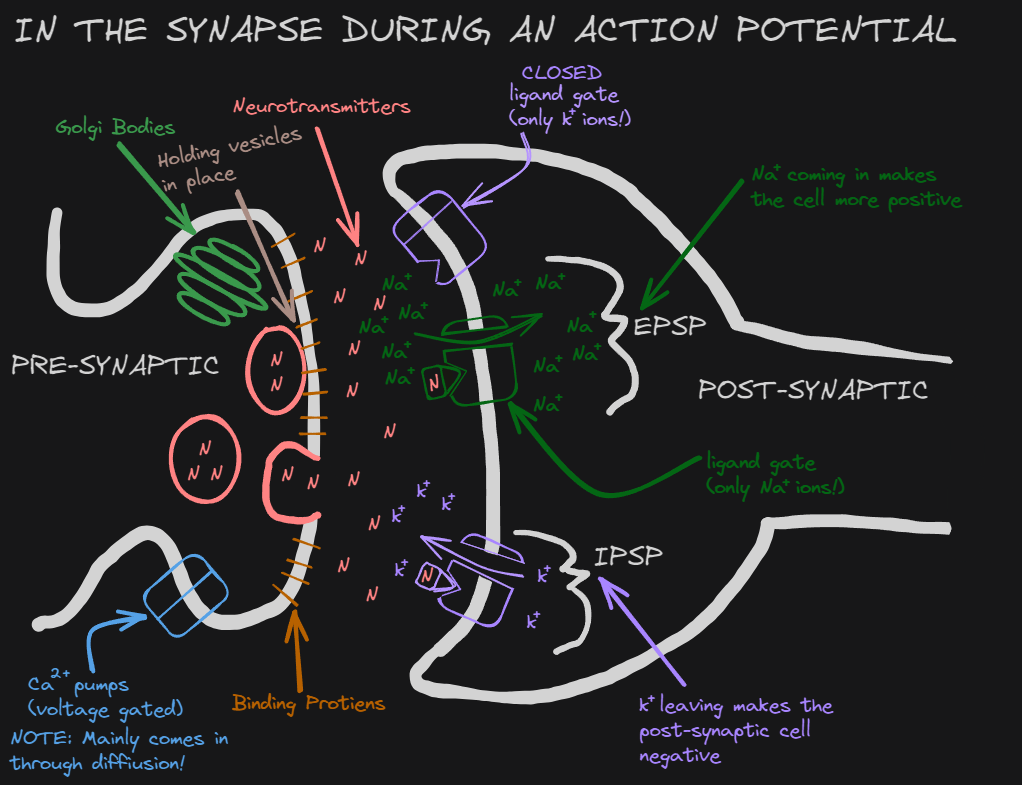
\includegraphics[width=.95\paperwidth,height=.95\paperheight,keepaspectratio]{excalidraw/neuron_synapse.png}
% \end{landscape}

% \begin{landscape}
%     \pagecolor{synapsebackground}
%     \pagestyle{plain}
%     \centering
%     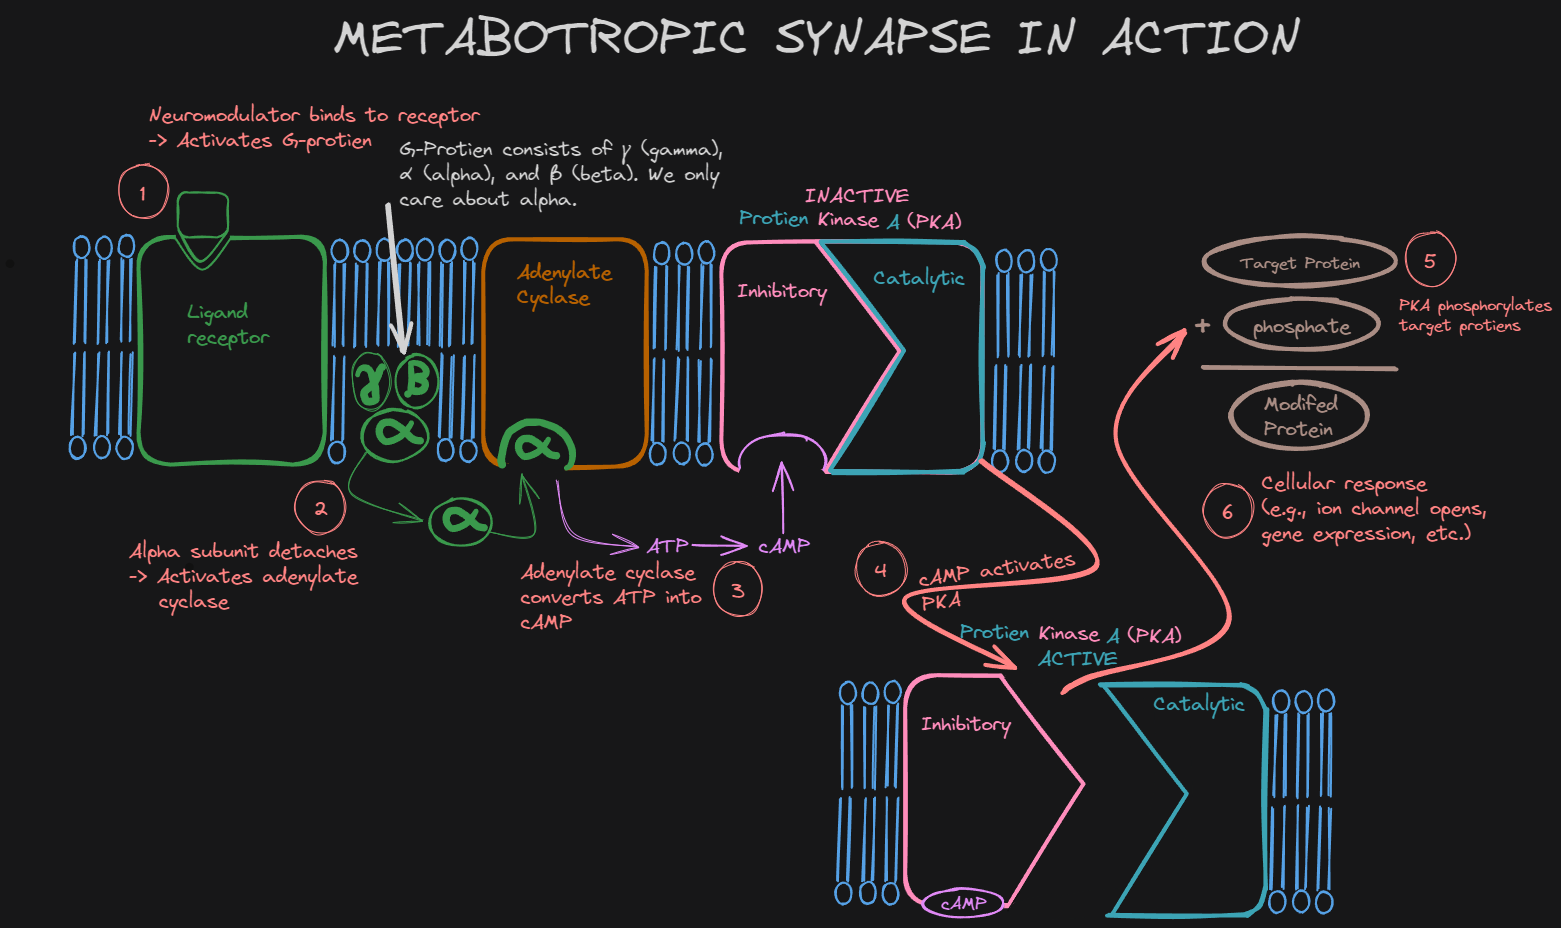
\includegraphics[width=.95\paperwidth,height=.95\paperheight,keepaspectratio]{excalidraw/metabotropic.png}
% \end{landscape}

% \pagecolor{draculabg}



\newpage
\begin{figure}[htbp]
    \centering
    \label{resting potential}
\begin{tikzpicture}
  % Labels for compartments
  \node at (-3,4.3) {\large \textbf{\underline{In}}};
  \node at (3,4.3) {\large \textbf{\underline{Out}}};
  \node at (-5.9,4.3) {\large \textbf{\underline{Permeability}}};

%   % Draw compartments as boxes
%   \draw (-5,-4) rectangle (-1,4); % Inside compartment
%   \draw (1,-4) rectangle (5,4);   % Outside compartment

  % Draw the membrane as a double line:
  % Left (solid) side denotes the negative (inside) and right (dotted) side the positive (outside)
  \draw[line width=1pt] (0.1,-4) -- (0.1,4);  
  \draw[dotted, line width=1pt] (-0.1,-4) -- (-0.1,4);

  % Place ion symbols on the "in" side (left) with relative sizes.
  % Here, potassium is large since it is more prevalent on the inside.
  \node (K_in) at (-3,2.5) {\huge \(\text{K}^{+}\)};
  \node (Na_in) at (-3,0) {\normalsize \(\text{Na}^{+}\)};
  \node (Cl_in) at (-3,-2.5) {\normalsize \(\text{Cl}^{-}\)};

  \node (P_K) at (-5.9,2.5) {\huge \(\text{P}\phantom{^{+}}\)};
  \node (P_K) at (-5.9,0) {\tiny \(\text{P}\phantom{^{+}}\)};
  \node (P_K) at (-5.9,-2.5) {\Large \(\text{P}\phantom{^{-}}\)};

  % Place ion symbols on the "out" side (right)
  % Here, sodium is made larger, etc.
  \node (K_out) at (3,2.5) {\normalsize \(\text{K}^{+}\)};
  \node (Na_out) at (3,0) {\huge \(\text{Na}^{+}\)};
  \node (Cl_out) at (3,-2.5) {\Large \(\text{Cl}^{-}\)};

  % Create nodes on the membrane for arrow connections
  \node (mem2_left) at (-0.5,0) {};
  \node (mem3_left) at (1.5,-2.5) {};
  \node (mem3_right) at (-1.5,-2.5) {};

  % Define arrow styles:
  \tikzset{
    diffusion/.style={->, >=Stealth, line width = 2pt, red},
    electric/.style={->, >=Stealth, line width = 2pt, blue}
  };

  % For each ion on the inside, draw two arrows (curved differently) going from the ion to the membrane.
  % The differences in the bending (and thus length) illustrate different magnitudes.
  % --- For K_in:
  \draw[electric, bend right=15] (K_in) to (K_out);
  \draw[diffusion, bend right=15, line width = 6pt] (K_out) to (K_in);
  % --- For Na_in:
  \draw[electric, bend left=15] (Na_out) to (mem2_left);
  \draw[diffusion, bend right=15] (Na_out) to (mem2_left);
  % --- For Cl_in:
  \draw[electric, bend right=15] (Cl_in) to (mem3_left);
  \draw[diffusion, bend right=15] (Cl_out) to (mem3_right);

  % Add a legend (key) to denote arrow styles.
  \node[draw, rectangle, right=1cm of K_out] (legend) {
    \begin{tabular}{ll}
      \textbf{Key:} & \\
      \tikz{\draw[diffusion, ->, >=Stealth, thick, red] (0,0) -- (1,0);} & Diffusion \\
      \tikz{\draw[electric, ->, >=Stealth, thick, blue] (0,0) -- (1,0);} & Electric \\
    \end{tabular}
  };
\end{tikzpicture}
\caption{The Resting Membrane Potential (RMP) of a Neuron}
\end{figure}

\begin{figure}[htbp]
    \centering
    \label{action potential}
\begin{tikzpicture}[scale=1.2]

    % Draw axes
    \draw[->, thick] (0,-4) -- (7,-4) node[right] {Time (ms)};
    \draw[->, thick] (0,-4) -- (0,3) node[above] {Voltage (mV)};

    % Draw threshold line at -55 mV and resting potential at -70 mV
    \draw[dashed] (0,-2.5) -- (7,-2.5) node[right] {Threshold (-55 mV)};
    \draw[dashed] (0,-3.5) -- (7,-3.5) node[right] {RMP (-70 mV)};
  
    % y-axis ticks and labels (scaling: 1 unit = 20 mV)
    \foreach \y/\label in {-3.5/{-70},-2.5/{-55}, -2/{-40}, -1/{-20}, 0/{0}, 1/{20}, 2/{40}} {
        \draw (0,\y) -- (-0.2,\y) node[left] {\label};
    }
    
    % x-axis ticks
    \foreach \x in {0,1,2,3,4,5,6} {
        \draw (\x,-4) -- (\x,-4.15) node[below] {\x};
    }
    
    % Draw action potential waveform using coordinates:
    % Points (x, y) where y = mV/20:
    % (0,-3.5):   Rest (-70 mV)
    % (1,-3.5):   Rest
    % (2,-2.75):  Threshold (-55 mV, since -55/20 = -2.75)
    % (3,2):      Peak depolarization (+40 mV, 40/20 = 2)
    % (4,-0.5):   Repolarization (-10 mV, -10/20 = -0.5)
    % (5,-4):     Hyperpolarization (-80 mV, -80/20 = -4)
    % (6,-3.5):   Return to rest (-70 mV)
    \draw[thick, horange] plot coordinates {
        (0,-3.5)
        (1,-3.5)
        (1.5,-3.5)
    };
    \draw[thick, horange, smooth] plot coordinates {
        (1.5,-3.5)
        (1.90,-2.55)
    };
    \draw[thick, horange] plot coordinates {
        (1.90,-2.55)
        (2,-2.5)
    };
    \draw[thick, horange, smooth] plot coordinates {
      (2,-2.5)
      (3,2)
      (4,-0.5)
      (5,-3.55)
      (6,-3.5)
    };

    % Add phase labels near the waveform
    \tikzset{
        circ/.style = {draw, circle, scale=0.7}
    };
    % Resting potential.
    \node[circ] at (1.3,-3.2) {1};
    % Opens sodium channels.
    \node[circ] at (1.75,-2.2) {2};
    % Potassium channels open.
    \node[circ] at (2.5,1.5) {3};
    % Sodium channels close.
    \node[circ] at (3.2,2.3) {4};
    % Potassium channels close.
    % \node[circ] at (6.1,-3.75) {5};
    
    \draw[decorate, decoration={brace, amplitude=5.5pt}]
    (5,-3.5) -- (6,-3.5);
    % Add text labels for phases
    \node at (2.2, 0) [rotate=78] {\textbf{Depolarization}};
    % The potassium is leaving the cell.
    \node at (4.2, 0) [rotate=287] {\textbf{Repolarization}};
    \node at (5.4, -3.1) {\textbf{Hyperpolarization}};

    % Arrow pointing hyperpolarization to -80 mv
    % \draw[->, thick] (7, -2) -- (4.93,-3.9) node[below] {};
  
  \end{tikzpicture}
    \caption{Action Potential Waveform}
\end{figure}

